\vspace{-4pt}
\subsection{Overview}
\label{sec:design}
\vspace{-4pt}

%\sysname\ performs file-level deduplication for a Docker registry.
%

%We designed \sysname\ so that the interface between the Docker clients and the
%registry remains unchanged.
%
%As such, no modifications to the Docker clients are needed.
%
%Below we describe how \sysname\ handles layer pushes and
%pulls at the registry side.
%
%For the sake of this paper, we explain only the main steps omitting smaller
%details.
%\Ali{Following text makes no sense.. what are you trying to explain??}
%\NZ{This part includes our architecture. Our architecture doesn't required many words to explain}
%
%Traditionally, Docker registry is a web server that serves Docker
%\texttt{pull} and Docker \texttt{push} requests.  Although Docker registry is a
%layer-level content addressable storage system holding all the images, it
%delegates storage to drivers which interact with either a local file system or
%a remote cloud storage like S3~\cite{xxx}, Microsoft Azure~\cite{xxxx}, OpenStack Swift~\cite{xxx}, and Aliyun
%OSS~\cite{xxx} as shown in Figure~\ref{fig:sys-overview}.
%Deduplication methods are implemented on remote cloud storage servers or data centers to
%transparently remove duplicates from the incoming data stream.

%proxy caches, or web/HTTP caches 
%Modern container registries such as Google Container Registry~\cite{GoogleContainerRegistry} use cloud storage as their backend Docker image storage systems. 
%Users push and pull Docker images to and from their repositories stored on cloud storage. 
%
%To facilitate a fast and high-availability service, container registries use regional private repositories across the world.  
%This geographical distribution allows users to store images close to their compute instances and experience a fast response time. 
%For example, IBM's Container Registry setup spans five regions~\cite{dockerworkload}. 

%caches are placed as close to the requesting client as possible,
%such caches are known as for the temporary
%storage of frequently requested data to reduce the server's lag.  They are
%typically deployed in a regional ISP or within a corporate network.

\sysname~seamlessly integrates 
%the management of 
caching and deduplication on the
backend storage system (\emph{backend dedup storage}) with Docker registries.
%
We address a set of unique challenges to enable this integration.
%
First, for caching layers, \texttt{pull} layer requests are difficult to
predict because layers are accessed infrequently.
In~\cref{sec:background},
%\arb{???}, 
we have observed that about half of the layers are not
accessed again for at least $1.3$~hours. Which means that if we
cache a layer, we may need to wait a long time before we observe a hit on that layer.  %(as discussed in~\cref{sec:background}).  
This is mainly 
because when a user pulls an image from the registry, the Docker daemon on the
requesting host will only pull the layers that are not locally stored.
%\Ali{I do not understand the following sentence.}
%Moreover, we have to consider that a user might deploy an applications on
%multiple machines, so it's not easy to predict when a user will access which layers. 
%%\Ali{The above statement is incorrect. You have to distinguish between GET layer requests
%that are issued after a (PUSH layer + GET manifest) request and a normal GET layer request.
%FAST paper only talk about case 1. Whereas you are generalizing that any GET layer request
%should have a precedent GET layer request which is wrong. We can make a case
%that not all GET layers requests have a precedent PUSH layer request but we can
%not say that it takes a few days, weeks, or even months for a user to make a pull
%layer request after a push layer request.}
%\NZ{I mean the first case, push beyond your trace collection time.}
%

Second, we can not deduplicate compressed layers. For deduplication, each layer
needs to be uncompressed, and only then can undergo file-level deduplication. Similarly,
to restore a layer, we need to fetch files from multiple servers, and only then compress
them in to a tar file to serve a \texttt{pull} layer request. 
%\arb{that can service the ??? request}\NZ{addressed}. 
This whole process can incur a 
considerable performance overhead on \texttt{pull} layer requests.
Deduplication also slows down
\texttt{push} layer requests because of its high demand for CPU, memory, I/O, and network resources.
%\Ali{Explain how push layer requests are not effected?}\NZ{fixed}

%\subsection{Design}
To address these issues, we propose a new registry design. The key feature of our design is a user-access-history-based prefetch algorithm that helps mitigate the performance degradation due to the 
backend dedup storage system (Figure~\ref{fig:sys-overview}). Based
on layer access pattern we observed in~\cref{sec:background} and user access history information,
\sysname precisely prefetch the layers that may be pulled shortly.
%has not been pulled in the requested repository
%and the prefetched 
%In this case, we can   
%a user's active time is predictable. 
%Thus, we leverage users' behavior, \ie
%when a user is most likely to be active, to drive layer evictions from the cache.

\begin{figure*}[t]
	\centering
		%\begin{minipage}{0.225\textwidth}
			\centering
			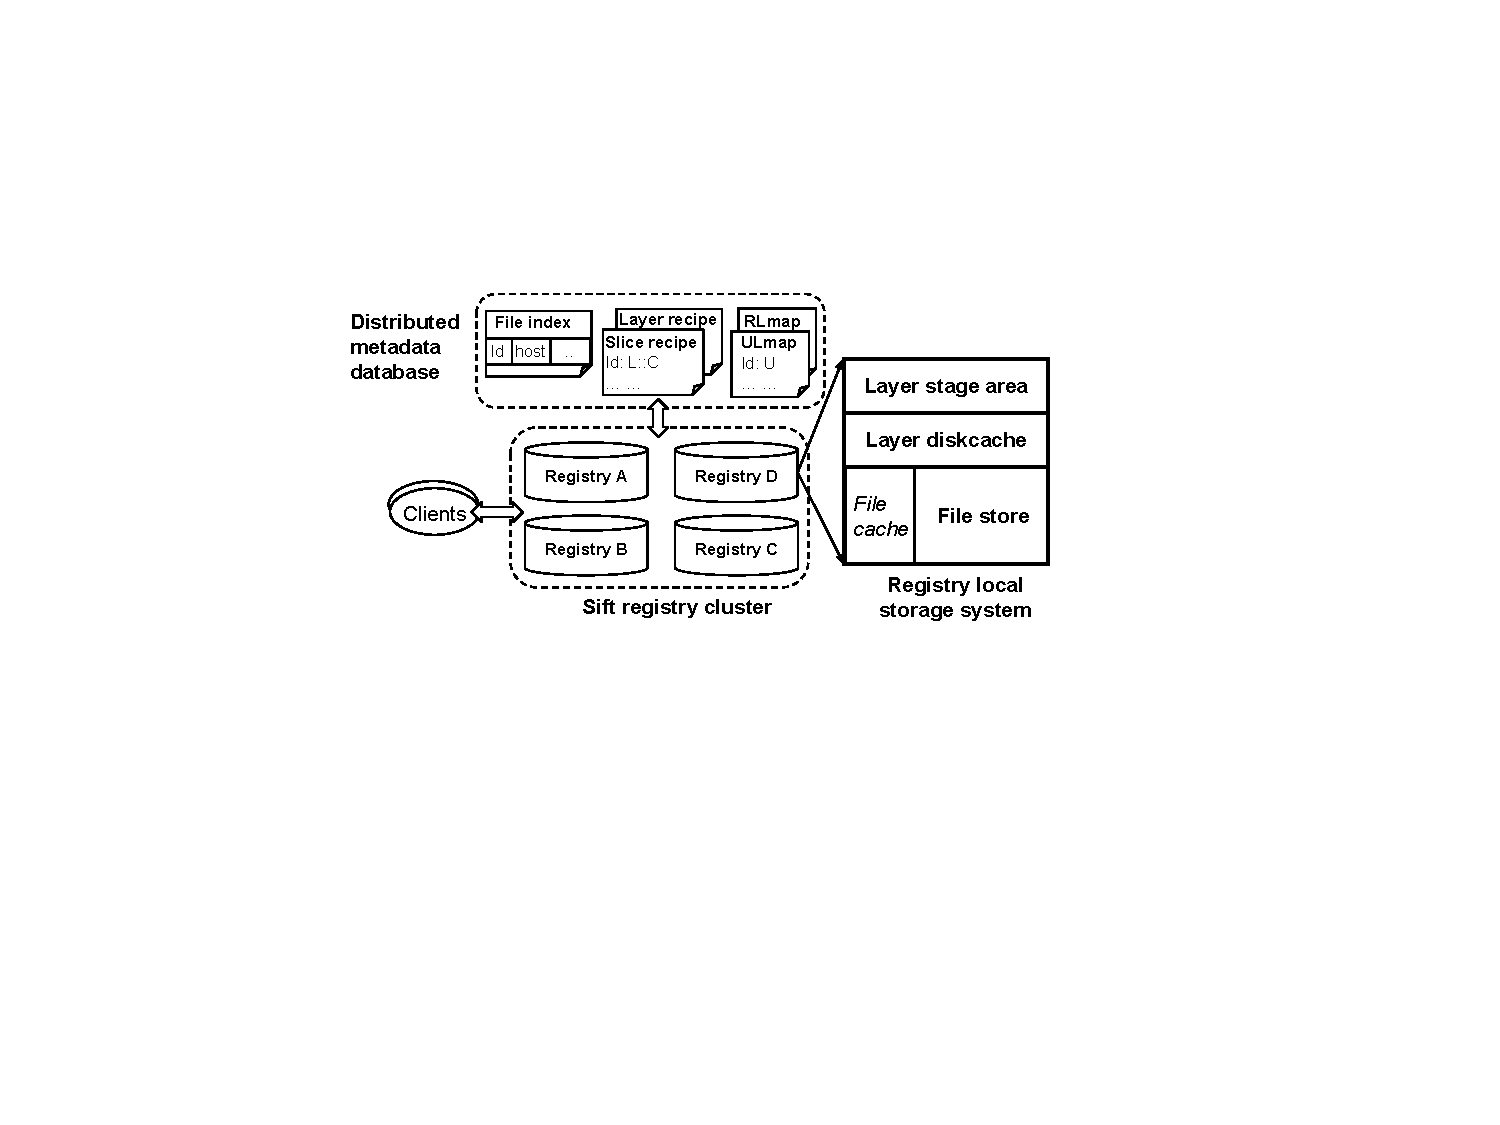
\includegraphics[width=0.9\textwidth]{graphs/sys-architecture.pdf}
%\vspace{-4pt}
			\caption{Architecture of \sysname.}
			%\label{fig:ref_count}
		%\end{minipage}
%	\begin{minipage}{0.225\textwidth}
%		\centering
%		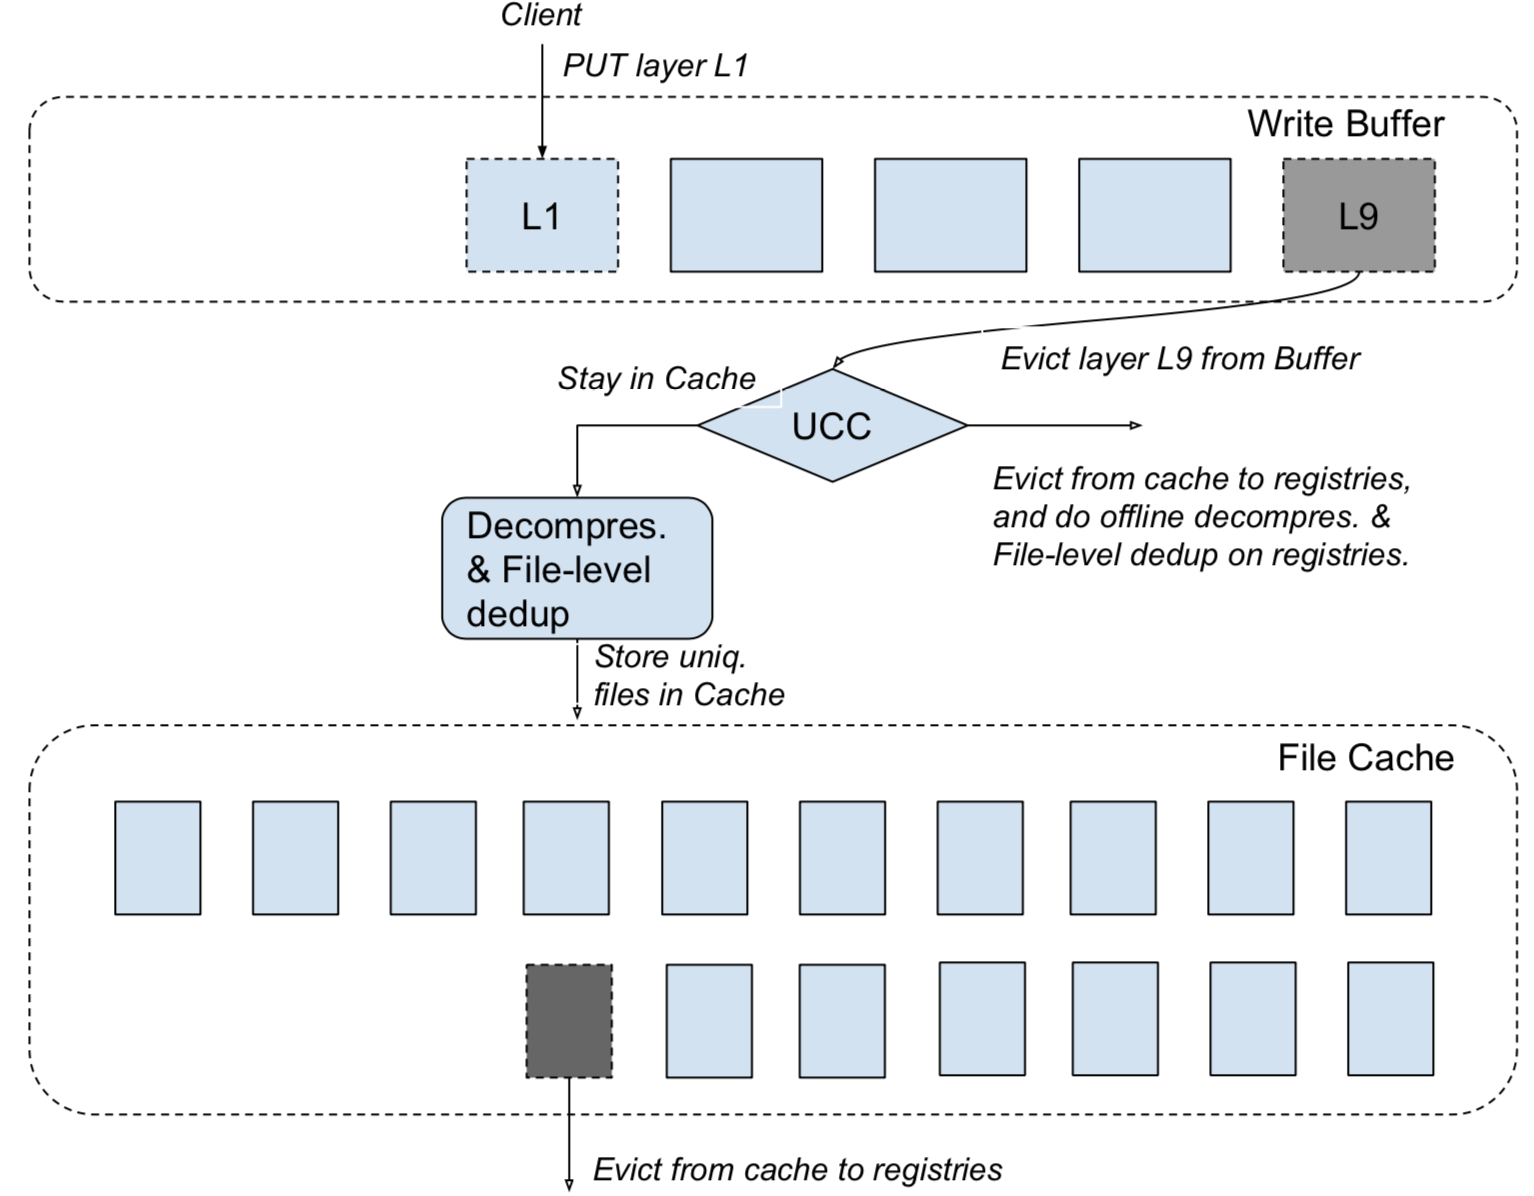
\includegraphics[width=1\textwidth]{graphs/slimmer-cache.png}
%		\caption{CDF of compress. and uncompress. layer size.}
%		\vspace{-3pt}
		\label{fig:sys-overview}
%\vspace{-4pt}
%	\end{minipage}
\end{figure*}


Considering that layer sizes are typically about several MB~\cite{dockerworkload}, 
a small main memory cache will be unable to accommodate
all prefetched layers for all active users. 
To address this issue, we 
create separate caches for layers and \emph{unique} files, called {\em layer buffer} and {\em file cache}, respectively. 
%Both caches comprise both
%main memory and flash memory.
%Layer buffer
%\arb{are main memory for one type and flash for the other type, or both for both types. I assumed both types of memory are used, and there are two caches. check previous sentence for correctness.}\NZ{addressed}
Note that, layers are  compressed tarballs and buffered in layer buffer, and 
%sent by users
 \emph{unique} files are uncompressed files from which duplicates have been removed and stored on flash-based storage. 
%We call compressed layer cache and \emph{deduped} files cache,
%\emph{layer buffer} and \emph{file cache}, respectively.
For 
cache evictions, we first evict inactive users' layers from the layer buffer.
Next, we \emph{dedup} the evicted layers, then store the \emph{unique} files
into the file cache (detailed in~\cref{sec:design_operations}). 
%the following operations: decompressing each evicted layer and comparing its
%containing files with the files that are already stored in the file cache,
%eliminating duplicate files, that is, only storing the unique files on flash
%storage.

When a user requests a
layer that is not present in the layer buffer, the request is forwarded to the
file cache (detailed in~\cref{sec:design_operations}). 
If a layer is also not found in the
file cache, the request is forwarded to the backend dedup storage system.
Note that after layer deduplication, unique files are
scattered across multiple servers. 
We define all the per-server files belonging to a layer as a {\em slice}. 
A server stores slices for many layers, and a layer is composed of slices stored on multiple servers.
To avoid the network latency caused by fetching slices from different servers and
assembling them into a whole compressed layer, we split a \texttt{pull} request 
into several~\texttt{pull slice}~requests. Those requests will then be
forwarded to all the backend servers that store the requested
layer's slices. 
After a~\texttt{pull slice}~request is received, each backend server compresses the slice 
and directly sends it back to the user.
We modify the Docker client
interface such that when it receives all the compressed slices, it can
decompress them into a single layer. 
Furthermore, compressing slices in parallel considerably lowers the layer compression latency,
since compression time depends on the size of the
uncompressed data.
%to cache layers and cache unique files after decompression and deduplication,
%respectively.  consists of a \emph{layer buffer} and a \emph{file cache}.  The
%layer buffer stores all the newly pushed layers in memory.  Although accessing
%memory is very fast, the size of main memory is limited. 
%All the slices for a layer are fetched in parallel for performance improvement.



 
